%% LaTeX2e class for student theses
%% sections/evaluation.tex
%% 
%% Karlsruhe Institute of Technology
%% Institute for Program Structures and Data Organization
%% Chair for Software Design and Quality (SDQ)
%%
%% Dr.-Ing. Erik Burger
%% burger@kit.edu
%%
%% Version 1.3.3, 2018-04-17

\chapter{Evaluation}
\label{ch:Evaluation}
In diesem Schritt, soll die bisherige Arbeit evaluiert werden und dabei gezeigt werden, dass die definierten Ziele erreicht werden konnten. Diese sollen mithilfe der Goal-Question-Metric (GQM) definiert werden. Erste Überlegungen sind in \autoref{tab:gqm} definiert.\par
Das Vorgehen der Evaluierung ist in \autoref{abb:ablauf_evaluierung} abgebildet. Zunächst wird das Evaluierungssystem aufzusetzen. Dazu zählt sowohl die Implementierung, als auch eine Modellierung des Systems. Dieses Evaluierungssystem soll die Anforderungen erfüllen, die in \autoref{sec:systemanforderungen} definiert wurden. Nachdem das System eingerichtet wurde, soll eine Performanzanalyse der naiven Implementierung und der Modellierung des Systems stattfinden, damit ein Referenzwert gegeben ist. Pro Durchlauf soll, im Anschluss, sowohl eine MOM-Modellierung, als auch ihre Implementierung in das Evaluierungssystem eingesetzt werden. Anschließend wird eine Performanzanalyse der Systemimplementierung und der -Modellierung durchgeführt werden. Schließlich werden die Ergebnisse ausgewertet.
\begin{figure}
\centering
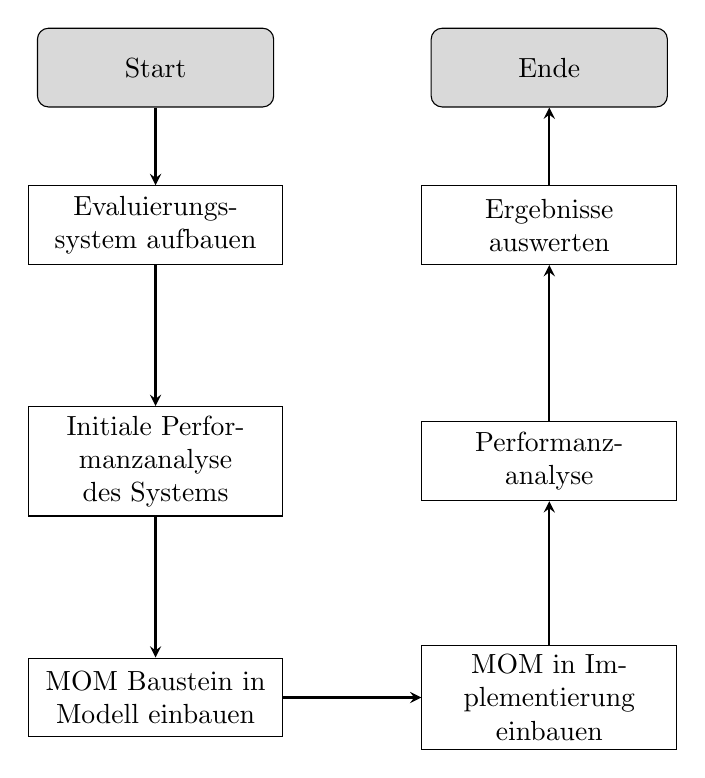
\begin{tikzpicture}[node distance=2cm]
\tikzstyle{startstop} = [rectangle, rounded corners, minimum width=3cm, minimum height=1cm,text centered, draw=black, fill=gray!30]

\tikzstyle{process} = [rectangle, minimum width=3cm, minimum height=1cm, text centered, text width=3cm, draw=black, fill=white!30]

\tikzstyle{decision} = [diamond, minimum width=1cm, minimum height=1cm, text centered, text width=2cm, draw=black, fill=white!30]
\tikzstyle{arrow} = [thick,->,>=stealth] 

\node (start) [startstop] {Start};
\node (pro1) [process, below of=start] {Evaluierungs-system aufbauen};
\node (pro2) [process, below of=pro1, yshift=-1cm] {Initiale Performanzanalyse des Systems};
\node (pro3) [process, below of=pro2, yshift=-1cm] {MOM Baustein in Modell einbauen};
\node (pro4) [process, right of=pro3, xshift=3cm] {MOM in Implementierung einbauen};
\node (pro5) [process, right of=pro2, xshift=3cm] {Performanz-analyse};
\node (pro6) [process, right of=pro1, xshift=3cm] {Ergebnisse auswerten};

%\node (dec1) [decision, right of=pro2, xshift=3cm] {Weitere MOMs?};

\node (ende) [startstop, right of=start, xshift=3cm] {Ende};


\draw [arrow] (start) -- (pro1);
\draw [arrow] (pro1) -- (pro2);
\draw [arrow] (pro2) -- (pro3);
\draw [arrow] (pro3) -- (pro4);
\draw [arrow] (pro4) -- (pro5);
\draw [arrow] (pro5) -- (pro6);
\draw [arrow] (pro6) -- (ende);
%\draw [arrow] (pro6) -- (dec1);
%\draw [arrow] (dec1) -- node[anchor=west] {ja} (pro3);
%\draw [arrow] (dec1) -- node[anchor=west] {nein} (ende);

\end{tikzpicture}
\caption{\label{abb:ablauf_evaluierung} Ablauf der Evaluierung.}
\end{figure}
\section{Goal-Question-Metric}
Die GQM-Methode \cite{gqm} spezifiziert Ziele für das zu validierende Konzept. Daraufhin werden zu den Zielen Fragen spezifiziert, mit denen die Erfüllung des Ziels überprüft werden soll. Schließlich werden Metriken festgelegt, durch die die Fragen beantwortet werden sollen. In \autoref{tab:gqm} sind erste Überlegungen festgehalten. Diese Überlegungen sind nicht vollständig und werden im Rahmen der Masterarbeit weiter ausgebaut.\par
Ein Ziel, das mithilfe dieser Masterarbeit erreicht werden soll, ist die Modellierung von MOMs in Palladio zu ermöglichen. Dafür wurden zwei Fragen definiert. Die erste Frage prüft ob sich MOMs überhaupt modellieren lassen. Die zweite Frage prüft die Modularität der MOM Bausteine. Das zweite Ziel ist, dass die Entscheidungsfindung, welche MOM verwendet werden soll, bereits zur Modellierungszeit und aus Architekturperspektive verbessert werden soll. Die dazu definierte Frage soll prüfen ob die Analyseergebnisse brauchbar, bzw. ob sich die Probleme einer Architekturentscheidung aus den Analyseergebnissen ableiten lassen. 
\begin{table}
  \begin{tabular}{|l|l|}
    \hline
    \multicolumn{2}{|l|}{Ziel 1} \\
    \hline
    Zweck & Ermögliche \\
    Qualitätskriterium & eine wartbare und wiederverwendbare Möglichkeit  \\ 
    Prozess & eine MOM zu modellieren \\
    Sicht & aus Architekturperspektive \\
   
    \hline \hline
    Frage 1 & Lassen sich MOMs modellieren? \\
    \hline
    Metrik & - Wie viele MOM Parameter konnten nicht modelliert werden? \\
    & - Wie viele Schritte müssen durchgeführt werden um eine neue \\
    & MOM zu modellieren\\
    \hline\hline
    Frage 2 & Wie modular sind die MOM Bausteine? \\
    \hline
    Metrik & - Wie viele Elemente müssen beim Austausch geändert werden? \\
    & - Min. Anzahl an Schritte um MOM auszutauschen \\
    \hline\hline
    \multicolumn{2}{|l|}{Ziel 2} \\
    \hline
    Zweck & Verbessere \\
    Qualitätskriterium & die Abwägung und Entscheidungsfindung  \\ 
    Prozess & beim Einsatz einer MOM \\
    Sicht & aus Architekturperspektive \\
    \hline \hline
    Frage 1 & Sind die Analyse Ergebnisse brauchbar? \\
    \hline
    Metrik & - Wie viel \% Abweichung zur naiven Modellierung/Implementierung? \\
    & - Wie viele Schritte müssen durchgeführt werden um Problem der \\
    & Architekturentscheidung aus dem Analyseergebnis abzuleiten? \\
    \hline
  \end{tabular}
	\caption{\label{tab:gqm} Ziele, Fragen und Metriken für die Evaluierung, nach der GQM-Methode}
\end{table}
\section{Systemanforderungen}
\label{sec:systemanforderungen}
Für die Masterarbeit werden zwei Systeme benötigt. Zum einen ein Experiment System um die verschiedenen MOMs vergleichen zu können und später die einzelnen Modellierungen an diesem kalibrieren zu können. Im Anschluss soll diese Modellierung in ein Evaluierungssystem eingebaut werden um zu zeigen, dass die zuvor definierten Ziele erreicht werden können. Im Rahmen des Proposals wurden Anforderungen an diese beiden Systeme erarbeitet.
\begin{itemize}
\item Das jeweilige System soll \textbf{Skalierung} erlauben. Dabei soll es zum einen möglich sein die Anzahl von Kommunikationspartnern zu erhöhen (\textit{horizontal}) als auch die Menge an Nachrichten die verschickt werden (\textit{vertikal}).
\item Weitere \textbf{Konfigurationen} wie Nachrichtengröße, reihenfolgentreue, Duplikate, etc. sollten möglich sein.
\item Die beiden Systeme sollen möglichst \textbf{reales System} darstellen.
\item Mindestens ein \textbf{Nachrichtenmodell} sollte unterstützt werden.
\item Es sollten \textbf{verschiedene Interaktionstypen} unterstützt werden, wie Many-To-Many, Many-To-One, etc.
\item Damit der Fokus der Masterarbeit auf den MOMs und ihrer Modellierung liegt, sollten die Systeme \textbf{bereits vorhanden} und implementiert sein.
\end{itemize}

\section{SPECJms2007}
Ein System das die in \autoref{sec:systemanforderungen} aufgestellten Anforderungen erfüllt ist das im SPECJms2007 Benchmark verwendete Testsystem \cite{Sachs2013}. Der Benchmark soll eine reale ereignisbasierte Anwendung darstellen und umfasst eine Reihe von verschiedener Interaktionen, die einen komplexen Mix aus Transaktionen darstellen, der sowohl Punkt-zu-Punkt- als auch Publish/Subscribe-Nachrichten einschließlich One-to-One-, One-to-Many- und Many-to-Many-Kommunikation umfasst. Bei dem System handelt es sich um ein Lieferkettenmanagement für eine Supermarktkette. Das System besteht aus vier Rollen, die in sieben verschiedenen Interaktionsmöglichkeiten miteinander kommunizieren können. Das System erlaubt verschiedene konfigurationen durch den Benutzer, wie die Nachrichtenröße oder die Skalierungsart. Für die Masterarbeit liegt sowohl die Implementierung des Benchmarks, als auch eine Modellierung aus einer früheren Arbeit von Christoph Rathfelder \cite{Rathfelder2013} vor. Dieses System soll als Experimentsystem verwendet werden um die verschiedenen MOMs zu vergleichen und zum kalibrieren der später erstellten Modellierung. 
\subsection{Szenarien}
Szenario 1 (SM sendet Anfrage an DC)

Szenario 2 (DC muss Waren auffüllen)
%- 3 szenarios aus Dissertation \\
%- 1. alle interaktionen und p2p uns p/s \\
%- 2. teilmenge der interaktionen und fokus auf p2p \\
%- 3. teilmenge der interaktionen und fokus auf p/s \\
\subsection{Anpassung des Modells}
Wo können Queues eingesetzt werden

Wo kann parametrisierung genutzt werden

wo muss anderer Ansatz gewaehlt werden?

\section{Modell vs Implementierung}


%\section{TIME}
%Ein weiteres System, das die Anforderungen aus \autoref{sec:systemanforderungen} erfüllt, ist das Transport Information Monitoring Environment (TIME) System \cite{time}. Dabei handelt es sich um ein System der Universität Cambridge. TIME soll ein reales Verkehrsüberwachungssystem darstellen. Es besteht aus mehreren verteilten Komponenten, die verschiedene Arten von Ereignissen senden bzw. empfangen. Die standardmäßige Middleware hat eine Peer-To-Peer Architektur, Punkt-zu-Punkt Kommunikation und unterstützt asynchronen Nachrichtenaustausch. Das System überwacht Autos mithilfe von Kennzeichenerkennung und soll den Verkehrsfluss optimieren. Diese Anwendung ist interessant, weil sie Daten von verschiedenen verteilten Sensoren und Systemen sammelt und integriert. Darüber hinaus enthält es Komponenten mit hohem und unterschiedlichem Ressourcenbedarf, wie z.B. der Kennzeichenerkennungsalgorithmus. Die Systemarchitektur ist sehr anpassungsfähig, wenn es darum geht, neue Komponenten hinzuzufügen oder die Verbindungen zwischen Komponenten oder deren Standort zu ändern. Was dazu führt, dass das hinzufügen und austauschen von verschiedenen MOMs möglich ist. Für die Masterarbeit liegt sowohl die Implementierung, als auch eine PCM-Modellierung des TIME Systems aus einer früheren Arbeit von Christoph Rathfelder \cite{Rathfelder2013} vor. Das TIME System soll für diese Masterarbeit als Evaluierungssystem dienen. Die Modellierung/Implementierung soll zunächst als Referenz für die Performanzanalyse dienen und im nächsten Schritt um verschiedene MOMs erweitert werden.